%===================================================================================
% Chapter: Design and implementation
%===================================================================================
\chapter{Diseño e implementación}
\label{chap:design-implem}
%===================================================================================
\section{Modelo general}
\label{sec:design}
El primer paso consiste en definir qué método utilizar para obtener una representación de la música (sobreponiéndose a la brecha semántica), que pueda ser utilizada para la recuperación semántica con consultas textuales.

Una de las estrategias de recuperación de información (con consultas textuales) utilizada extensamente, como se ha mencionado anteriormente, es mediante metadatos. Se debe recordar que dicha estrategia requiere que las canciones contengan metadatos curados (que no es muy práctico en los escenarios actuales donde la multimedia se genera en grandes cantidades, y libremente). Además, como segunda desventaja, la información conocida sobre las canciones estaría limitada al conjunto fijo de metadatos que se predefinan. 

Si se extraen los metadatos (\textit{tags}, \textit{features}) automáticamente con modelos de \textit{Machine Learning} de clasificación y auto-tagging, se hace frente al primer problema mencionado: cómo hacer que todas las canciones tengan metadatos, sin requerir una cantidad de trabajo humano irrealista. Dado que los \textit{tags} se extraen automáticamente, se abre una ventana a contrarrestar la segunda desventaja, ya que la cantidad de tags dependería de la cantidad de modelos de \textit{Machine Learning}. Esto incluso permite que el conjunto no sea fijo. Con el costo de reprocesar la base de datos, se hace posible actualizar y añadir valores.

Otra estrategia, que ha sido analizada por las escasas investigaciones en el tema, es diseñar un modelo para convertir la música al espacio del lenguage natural, o convertir las descripciones textuales y la música a un espacio compartido. El problema fundamental de este acercamiento es que requiere un conjunto bastante grande de pares texto-música, lo suficientemente diverso y abarcador para maximimar la generalización del modelo. La inexistencia de dichos datasets \cite{Simonetta2019MultimodalMI, Huang2022MuLanAJ, Manco2022ContrastiveAL}, en conjunto con las dificultades de requerimientos computacionales; no permiten realizar el entrenamiento necesario para implementar esta estrategia. 

La propuesta de extraer los \textit{features} automáticamente trabaja bajo la premisa de que el campo de MIR se ha desarrollado en tareas de clasificación y auto-tagging lo suficiente para ser competitivo con metadatos hechos a mano, relativo al esfuerzo que conlleva cada uno. % TODO specify a little more on our proposal

Para garantizar que el sistema de recuperación tenga en cuenta la similitud semántica, se propone utilizar un acercamiento con \textit{Sentence BERT} (sec. \ref{sec:semantic_embedd}) para comparar las consultas con las descripciones de la música. Los enfoques tradicionales en SRI para mantener la significación semántica, suelen requerir estructuras complejas y un largo tiempo de preprocesamiento o de ranking (como Latent Semantic Analysis (LSA) \cite{Foltz1996LatentSA}). Con el auge de los modelos de lenguaje (alrededor de los últimos de cinco años) y su capacidad de capturar significado semántico y relación contextual; se ha abierto el camino para combinar la eficiencia del modelo vectorial con bolsa de palabras y el aumento en precisión de los modelos como LSA. 
% TODO explain the relationship between language models and the combination 

Dado que SBERT captura el \textit{embedding} de un texto, y que el \textit{framework} de extracción de \textit{features} lo que devuelve es una lista de \textit{tags}, es necesario convertirla a texto en lenguaje natural.  

La tarea de generación de texto a partir de tablas (\textit{table-to-text generation}) consiste en tomar una tabla estructurada como entrada y producir una descripción en lenguaje natural \cite{Yang2021TableTT}. Tiene buenas perspectivas de aplicación en la comunicación con humanos de manera comprensible y natural, como en la generación de informes financieros, informes médicos, etc. 

La mejor alternativa que se encontró para convertir los \textit{features} en texto fue utilizar \textit{TableGPT: few-shot Table-to-text generation with Table Structure Reconstruction and Content Matching}. TableGPT \cite{Gong2020TableGPTFT} se enfoca en generar texto de alta fidelidad para la generación de texto a partir de tablas con un número limitado de pares de entrenamiento. Abordando la brecha entre la entrada (tablas estructuradas) y la entrada de GPT-2 (lenguaje natural); TableGPT intenta transformar naturalmente las tablas estructuradas en lenguaje natural. Sin embargo, este modelo no se encuentra accesible para ser utilizado directamente con inferencia. Para hacer uso de TableGPT sería necesario recrear todo su proceso de entrenamiento. Pero en el desarrollo de la investigación no se contó con los recursos computacionales para efectuarlo.

Entonces las propuestas factibles son: 
\begin{itemize}
    \item utilizar GPT-2 directamente para generar descripciones a partir de la lista de metadatos
    \item crear una oración con fuerza bruta, por ejemplo para el género: \\" The music genre sounds like <\textit{genre classification}>. "
    \item utilizar un aceramiento similar a MusCALL \cite{Manco2022ContrastiveAL}, de concatenar tags en un oración
\end{itemize}
La primera requiere hacer \textit{prompt engineering} y no garantiza fidelidad con los datos extraídos. Mientras que las otras dos resultarían en descripciones que distan de la forma en que las personas realmente realizan consultas. 

Teniendo en cuenta todo esto, se propone intentar las tres estrategias de convertir \textit{tags} en descripciones y comparar los resultados con las tres alternativas.\\

En resumen, la implementación del prototipo objetivo implica desarrollar una plataforma que permita realizar consultas en lenguaje natural sobre una base de datos de música y obtener resultados con significado semántico. La propuesta del presente trabajo (fig. \ref{fig:corpus_embeddings}) consiste en:
\begin{itemize}
    \item un sistema de extracción de \textit{features} compuesto por modelos de clasificación de música (incluyendo \textit{features} de bajo y alto nivel).
    \item las características extraídas, entonces, son convertidas en descripciones utilizando las tres alternativas mencionadas anteriormente, obteniendo tres corpus de \textit{captions}.
    \item finalmente las descripciones serían procesadas con SBERT para generar los \textit{embeddings} que se utilizan en el sistema de recuperación.
\end{itemize}
\begin{figure}[h]
	\centering
	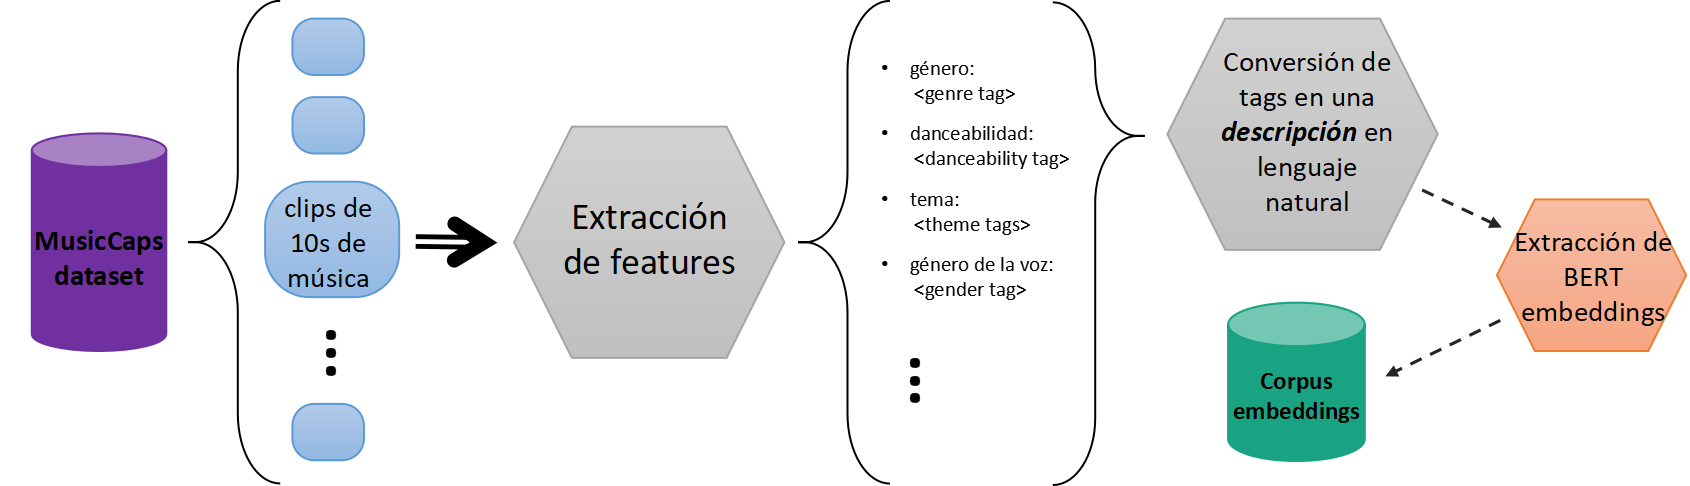
\includegraphics[width=\textwidth]{Graphics/corpus_embeddings.png}
	\caption{Diseño propuesto.} 
    \label{fig:corpus_embeddings}
\end{figure}
En el apartado de recuperación de información, el sistema consiste en recopilar la consulta del usuario, generar el vector de \textit{embedding} con SBERT y encontrar las canciones más similares comparando el vector con el corpus de \textit{embeddings}, utilizando similitud de coseno. En la imagen \ref{fig:sri_design} se observa el diseño del SRI. 
\begin{figure}[h]
	\centering
	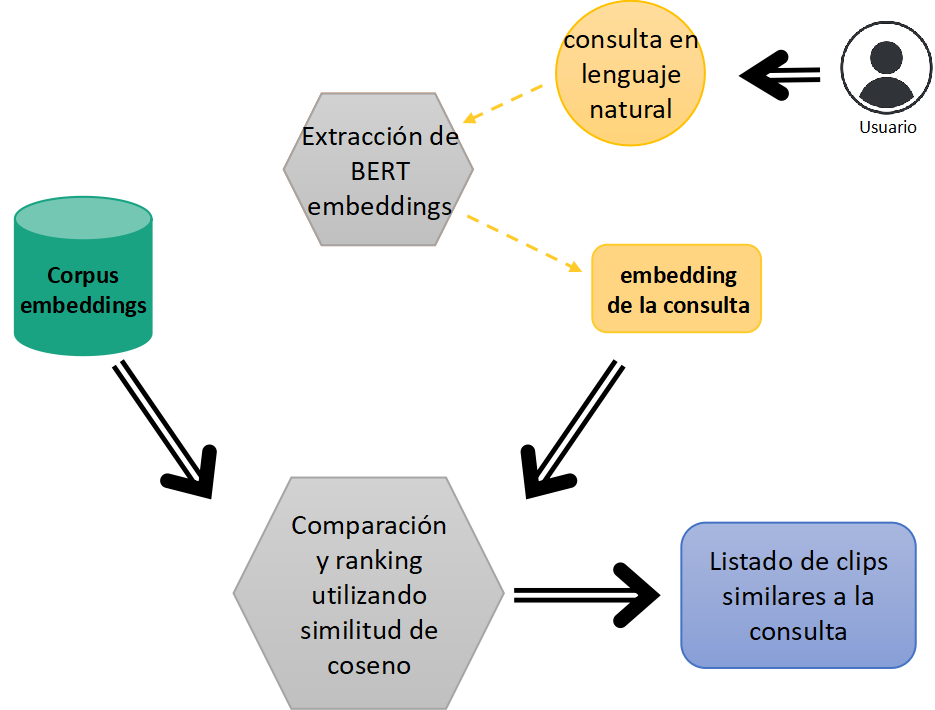
\includegraphics[width=0.6\textwidth]{Graphics/SRI.png}
	\caption{Sistema de recuperación utilizando \textit{Sentence BERT embeddings}.} 
    \label{fig:sri_design}
\end{figure}
\section{Detalles de implementación}
\label{sec:implementation}
\subsection{Extracción de \textit{features}}
\label{subsec:essentia}
La arquitectura del sistema de extracción de \textit{features} fue relativamente sencilla de implementar. Un sistema de clases que heredan de la clase abstracta \textit{FeaturesExtractor}. \\
Las propiedades incluyen: una lista de las etiquetas de clase posibles de cada modelo; \textit{feature\_description} que retorna una oración en lenguaje natural describiendo una etiqueta de clase; \textit{feature\_tags\_description} retorna un \textit{tag}/metadato describiendo una etiqueta de clase. Además de la función \textit{extract\_feature}, que recibe un clip de música y retorna el(los) \textit{feature(s)} extraídos con el modelo específico. \\
Los modelos utilizados, para probar y evaluar el diseño son parte de los que provee la biblioteca \textit{essentia} en conjunto con \textit{tensorflow} \cite{alonso2020tensorflow}. Se utilizaron 9 modelos : \href{https://essentia.upf.edu/models.html#genre-discogs400}{Genre Discogs400}, \href{https://essentia.upf.edu/models.html#mtg-jamendo-genre}{MTG-Jamendo genre},  \href{https://essentia.upf.edu/models.html#danceability}{Danceability}, \href{https://essentia.upf.edu/models.html#mood-happy}{Mood Happy}, \href{https://essentia.upf.edu/models.html#mood-relaxed}{Mood Relaxed}, \href{https://essentia.upf.edu/models.html#mood-sad}{Mood Sad}, \href{https://essentia.upf.edu/models.html#mtg-jamendo-mood-and-theme}{MTG-Jamendo mood and theme}, \href{https://essentia.upf.edu/models.html#mtg-jamendo-instrument}{MTG-Jamendo instrument} y \href{https://essentia.upf.edu/models.html#voice-gender}{Voice gender}.

Los modelos de clasificación de \textit{essentia} requiren que el audio sea convertido a \textit{embeddings} para recibirlos como entrada, y fue utilizado para ello el modelo \textit{Discogs-EffNet} \footnote{\href{https://essentia.upf.edu/models.html}{https://essentia.upf.edu/models.html}}.

En \textit{musiccaps-subset-feat.csv} \footnote{\href{https://github.com/NileyGF/Busqueda-semantica-en-audios.-Tesis/blob/main/src/data/musiccaps-subset-feat.csv}{https://github.com/NileyGF/Busqueda-semantica-en-audios.-Tesis/blob/main/src/data/musiccaps-subset-feat.csv}} (tabla \ref{tab:feat.csv}) se puede observar el subconjunto utilizado de MusicCaps con los \textit{features} extraídos, además de la información originaria del dataset sobre cada clip. Este proceso, en una computadora con 24 GB de RAM y procesador Intel Core i7-4710HQ, tomó alrededor de 18 horas para terminar con los alrededor de 3800 clips.
\begin{table}[h]
    \tiny
    \centering
    \begin{tabular} { | p{5em} | p{4em} | p{6em} | p{4em} | p{4.5em} | p{4.5em} | p{4em} | c | p{4.8em} | p{4em} |}
    \hline
     \multicolumn{3}{|c|}{ } & \multicolumn{7}{|c|}{Extracted features} \\
    \hline
        ytid    & aspect list & caption &Discogs 400 genre & MTG Jamendo genre &danceability & happy & ... &instruments & voice gender\\ 
    \hline
    -0Gj8-vB1q4 &['low quality', ... , 'ballad'] &"The low quality recording ... like something you would hear at Sunday services." & 
                                    Stage \& Screen---Soundtrack & classical &not danceable &non happy & ... & ['piano', 'violin', 'cello'] & female \\
    \hline
    -0SdAVK79lg &['guitar song', 'piano backing', ... , 'no voice'] &"This song features an electric guitar ... This song can be played in a coffee shop."  
                                &Blues---Delta Blues & pop &not danceable & non happy & ... & ['guitar', 'acousticguitar', 'bass'] & female \\
    \hline
    \multicolumn{10}{|c|}{ \textbf{.....} } \\ 
    \hline
    \end{tabular}
    \caption{Fragmento del archivo musiccaps-subset-feat.csv}
    \label{tab:feat.csv}
\end{table}

\subsection{Conversión de tags en una descripción en lenguaje natural}
\label{subsec:feat-to-text}

Como fue mencionado en la sección \ref{sec:design}, la idea era implementar tres alternativas para obtener descripciones a partir de los \textit{features} extraídos anteriormente. \\

\textbf{Utilizar GPT-2 con \textit{prompt engineering}}\\
Se intentó unas decenas de prompts utilizando el modelo de completamiento de texto de GPT-2 \cite{radford2019language, HggFaceGPT2}. Sin embargo, no se obtuvo resultados aceptables con ningún de ellos. Teniendo en cuenta dichos resultados se probó con GPT-3.5, desde la página de Open-AI; y esta vez si se observaron buenas descripciones, aunque no completamente fieles, como es de esperar de estos modelos. Sin embargo, no es factible realizar casi 4000 peticiones, ya que a diferencia de GPT-2, GPT-3.5 no es tan accesible. Por lo tanto esta alternativa tuvo que ser descartada.\\

\textbf{Crear una oración con fuerza bruta}\\
Utilizando la propiedad \textit{feature\_description}, se generó una oración por cada \textit{feature} extraído, por cada uno de los clips en el dataset. La concatenación de dichas oraciones en un texto constituyó el corpus de descripciones. \\
Ejemplos de la metodología para crear las oraciones:
\begin{itemize}
    \item MTG-Jamendo genre: " The music genre sounds like <\textit{genre classification}>. "
    \item Mood Relaxed: $"$ Its sound is >\textit{relaxing/not relaxing}>. "
    \item MTG-Jamendo instrument: " You can hear the sounds of <\textit{comma separated top instruments}>. "
    \item Voice gender: " There is a <\textit{female/male}> voice. "
\end{itemize}
Aprovechando la libertad al diseñar el sistema de recomendación, se propuso realizar un segundo corpus de descripciones conteniendo las oraciones separadas además del texto resultado de la concatenación. De forma que este corpus extendido tiene 10 descripciones (que posteriormente son transformadas en \textit{embeddings}) por cada clip (una oración por cada uno de los 9 \textit{features} y el texto completo). Esta idea surge para comparar que ofrece mejores resultados en la recuperación con \textit{embeddings}: una consulta en forma de texto largo u oraciones más cortas, pero repetitivas a través del conjunto de datos.\\

\textbf{Concatenar \textit{features} sin intentar que parezca una oración humana}\\
Utilizando la propiedad \textit{feature\_tags\_description}, se creó una `oración' por cada clip, donde el valor de cada \textit{feature} es separado del siguiente por un `; '. En algunos, la propiedad modifica ligeramente el valor resultante del modelo de clasificación. Por ejemplo, tiene más sentido semántico utilizar \textit{``\{female/male\} voice ''}, que simplemente \textit{``\{female/male\}''}.\\

En \textit{musiccaps-subset-descriptions.csv} \footnote{\href{https://github.com/NileyGF/Busqueda-semantica-en-audios.-Tesis/blob/main/src/data/musiccaps-subset-descriptions.csv} {https://github.com/NileyGF/Busqueda-semantica-en-audios.-Tesis/blob/main/src/data/musiccaps-subset-descriptions.csv } } (tabla \ref{tab:descriptions.csv})  se pueden observar las descripciones de cada clip, tanto en formato de oraciones procesadas, como de tags concatenados. 
\begin{table} [h]
    \tiny
    \centering
    \begin{tabular} { | p{5em} | p{4em} | p{6em} | p{4em} | p{4em} | c | p{4em} | p{6em} | p{6em} |}
    \hline
     \multicolumn{3}{|c|}{ } & \multicolumn{4}{|c|}{Extracted features} & \multicolumn{2}{|c|}{Descriptions} \\
    \hline
        ytid    & aspect list & caption &Discogs 400 genre & MTG Jamendo genre & ... & voice gender & description & tags description \\ 
    \hline
    -0Gj8-vB1q4 &['low quality', ... , 'ballad'] &"The low quality recording ... like something you would hear at Sunday services." & Stage \& Screen---Soundtrack & classical & ... & female &"The music genre is considered to be Stage \& Screen, Soundtrack ... There is a female voice. " &"Stage \& Screen, Soundtrack; classical; ... ; female voice."\\
    \hline
    -0SdAVK79lg &['guitar song', 'piano backing', ... , 'no voice'] &"This song features an electric guitar ... This song can be played in a coffee shop."  & Blues---Delta Blues & pop & ... & female &"The music genre is considered to be Blues, Delta Blues ... There is a female voice. " &"Blues, Delta Blues; pop; ... ; female voice."\\
    \hline
    \multicolumn{9}{|c|}{ \textbf{.....} } \\ 
    \hline
    \end{tabular}
    \caption{Fragmento del archivo musiccaps-subset-descriptions.csv}
    \label{tab:descriptions.csv}
\end{table}

\subsection{Extracción de \textit{embeddings} de BERT}
\label{subsec:bert-embedd-extr}

Cada uno de los 3 corpus de descripciones fueron posteriormente procesados para crear un vector de \textit{embeddings} por cada clip utilizando el modelo de la biblioteca \textit{transformers} de \textit{HuggingFace}: \textbf{bert-base-uncased}. El proceso consiste en tokenizar el texto con la función \textbf{BertTokenizer} de \textit{transformers}: \\
\begin{lstlisting}[language=Python]
preprocess_tokens = "[CLS]" + text + "[SEP]"
\end{lstlisting} 
Luego se transforma el texto tokenizado a \textit{embeddings}, utilizando la biblioteca \textit{torch} y el modelo de BERT. Al finalizar se guarda la lista de embeddings como un archivo binario, que no se encuentran en el repositorio debido a que ocupan relativamente bastante espacio.

El primer corpus de \textit{embeddings} tomó en computarse, en una computadora con 24 GB de RAM y procesador Intel Core i7-4710HQ, alrededor de 2 horas. El segundo, que consiste en una extensión del primero con 10 veces la cantidad de \textit{embeddings}, tomó entre 14 y 15 horas de procesamiento. El tercer corpus, constituido por la concatenación de tags tomó entre 1 y 2 horas en terminar.

Como último detalle, en esta parte de la implementación al finalizar de procesar cada corpus se creó un diccionario que establece por cada \textit{embedding} a que clip corresponde. Esto es particularmente importante en el caso del segundo, ya que existen 10 \textit{embeddings} por cada clip.

\subsection{Recuperación de Información. Comparación y ranking}
\label{subsec:IR-process-query}

El método de obtener la música más cercana consiste en obtener un vector de \textit{embeddings} a partir del texto de la consulta, utilizando el mismo proceso descrito anteriormente en  \ref{subsec:bert-embedd-extr}. Luego se compara dicho vector con cada uno de los \textit{embeddings} en el corpus (solo se emplea uno de los tres), utilizando la similitud del coseno entre el ángulo de los vectores. Finalmente se ordenan descendentemente, ya que el coseno es mayor entre vectores más cercanos. Se puede especificar cuantos resultados obtener: todos, o solo los $k$ más similares a la consulta. 

Después de ordenar los \textit{embeddings} se busca la correspondencia entre ellos y los clips, de forma que la relevancia de un clip es la relevancia del primer \textit{embedding} correspondiente a él (o sea, el de mayor valor de coseno). Esto es particularmente importante para el segundo corpus y cualquier otro que se pueda diseñar eventualmente donde a un clip le corresponda más de un vector de \textit{embeddings} (por ejemplo, si la descripción contiene más de 512 \textit{tokens} no puede ser procesada con BERT, y puede solucionarse dividiéndola en varias subdescripciones más cortas).

